\documentclass{article}
\usepackage{hyperref}
\usepackage{listings}
\usepackage{color}
\usepackage{xcolor}
\usepackage{geometry}
\usepackage{graphicx}
\usepackage{amsmath}
\usepackage{caption}
\usepackage{subcaption}
\geometry{margin=1in}
\pdfminorversion=6

\newcommand\TODO[1]{\textcolor{red}{TODO: #1}}

\newcommand\header[2]{
    \begin{center}
        {\large
        UCSD CSE 168 Assignment #1: \\
        \vspace{0.3cm}
        \Large
        #2}
    \end{center}
}

\definecolor{dkgreen}{rgb}{0,0.6,0}
\definecolor{gray}{rgb}{0.5,0.5,0.5}
\definecolor{mauve}{rgb}{0.58,0,0.82}
\lstset{frame=tb,
        aboveskip=3mm,
        belowskip=3mm,
        showstringspaces=false,
        columns=flexible,
        basicstyle={\small\ttfamily},
        numbers=none,
        numberstyle=\tiny\color{gray},
        keywordstyle=\color{blue},
        commentstyle=\color{dkgreen},
        stringstyle=\color{mauve},
        breaklines=true,
        breakatwhitespace=true,
        tabsize=2
}

\hypersetup{colorlinks=true}

\usepackage{xcolor}

\begin{document}

\header{3}{Indirect lighting and BRDFs}
In this homework, we will implement an actual \href{https://en.wikipedia.org/wiki/Path_tracing}{path tracing} algorithm. We are close to finishing the RTRYL book!

\section{Diffuse interreflection}
So far in our code, we seem to be treating the diffuse and specular surfaces separately: diffuse surfaces gather contributions from lights, and specular surfaces trace out rays that collect color from other surfaces (and \lstinline{plastic} is a mixture of them). In real world, diffuse surfaces also collect colors from other surfaces. We will implement this in this part.

In the previous homeworks, we do something like this:
\begin{lstlisting}[language=python]
\begin{lstlisting}[language=python]
def radiance(scene, ray, rng):
  if (ray intersect scene):
    # [emission] add emission of the intersected shape
    # ...
    # [direct_lighting] loop over lights, sample them, and sum over their contributions
    # ...
    # [scattering] recursively tracing the ray by calling radiance
    if (hit a metal or plastic):
      # recursively trace a ray towards the mirror reflection direction
      # ...
  else:
    return scene.background_color
\end{lstlisting}

In this homework, we will temporarily suspend the direct lighting code -- we will add it back later in the next homework.

We will extend the scattering code to handle diffuse materials in this homework. As with the case of area light, conceptually this is simple: instead of always tracing rays towards the mirror reflection direction, we randomly sample rays at different directions and accumulate contributions (\href{https://raytracing.github.io/books/RayTracingInOneWeekend.html#diffusematerials}{Chapter 8} of RTOW describes one approach to do this). But what distribution should we use, and how do we weigh different directions? That's where we need to do the math.

Remember the area light integral, where we integrate over all points on a light source $S$:
\begin{equation}
\int_{x \in S} f(x) \mathrm{d}A(x) = \int_{x \in S} \frac{K_d \cdot \max\left(n_s \cdot l, 0\right)}{\pi} \cdot \frac{I \max\left(-n_x \cdot l, 0\right)}{d^2} \cdot \text{visibility} \cdot \mathrm{d}A(x),
\label{eq:area_light}
\end{equation}
where $K_d$ is the diffuse reflectance, $n_s$ is the normal at the shading point, $l$ is the unit vector pointing from the shading point towards $x$, $n_x$ is the geometric normal at point $x$ on the light source, and $d$ is the distance between the shading point and $x$.

We will derive the equations of diffuse interreflection from Equation~\eqref{eq:area_light}. Let's play with an idea: what if everything is light source? We will figure out how to assign the intensity $I$ later. Apart from the intensity, all we need to change is the integration domain: instead of integrating a particular light source $S$, we integrate over all surfaces $\mathcal{M}$. Next, since we are tracing rays, we want to deal with directions, instead of points on surfaces. We achieve this using a \emph{change of variable} (again!) -- instead of integrating over position $x$, we integrate over direction $\omega$:
\begin{equation}
\int_{x \in \mathcal{M}} \frac{K_d \cdot \max\left(n_s \cdot l, 0\right)}{\pi} \cdot \frac{L \max\left(-n_x \cdot l, 0\right)}{d^2} \cdot \text{visibility} \cdot \mathrm{d}A(x) = 
\int_{\omega \in \Omega} \frac{K_d \cdot \max\left(n_s \cdot \omega, 0\right)}{\pi} \cdot L \cdot \mathrm{d}\omega.
\label{eq:area_light_solid_angle}
\end{equation}
Firstly, we have replaced $S$ with $\mathcal{M}$ and $I$ with $L$ to emphasize that things are different now.
Also note that $\omega = l$.
Here, the measure $\mathrm{d}\omega$ is often called the \href{https://en.wikipedia.org/wiki/Solid_angle}{solid angle} -- it represents an infinitesimal area of a point on a unit sphere. You will notice that the equation gets a lot simpler after we switch to the solid angle measure. This is because the Jacobian of the change of variable is exactly the reciprocal of $\frac{\max\left(-n_x \cdot \omega, 0\right)}{d^2} \cdot \text{visibility}$ (see \href{https://raytracing.github.io/books/RayTracingTheRestOfYourLife.html#samplinglightsdirectly/gettingthepdfofalight}{Chapter 9.1} of RTRYL for an explanation). Intuitively, the Jacobian captures the ratio of area on the surface $\mathcal{M}$ and its projcted area on a unit sphere (if it is not blocked).

We still need to decide what is the color $I$. Remember in the mirror case, we recursively trace rays to determine the color. We can do the same thing for diffuse surfaces too!
\begin{equation}
L = \int_{\omega \in \Omega} \frac{K_d \cdot \max\left(n_s \cdot \omega, 0\right)}{\pi} \cdot L \cdot \mathrm{d}\omega.
\end{equation}
This is however vacuous, because there is no \emph{base case} for this recursion. We will instead add the emission whenever we hit a light source\footnote{The infinite recursion defined in Equation~\eqref{eq:diffuse_rendering_equation} is actually mathematically well-behaved, as long as $K_d < 1$ for all channels. The reason is that after each bounce, some energy will be absorbed by $K_d$, and eventually the ray will carry zero energy.}:
\begin{equation}
L = L_e + \int_{\omega \in \Omega} \frac{K_d \cdot \max\left(n_s \cdot \omega, 0\right)}{\pi} \cdot L \cdot \mathrm{d}\omega.
\label{eq:diffuse_rendering_equation}
\end{equation}
We have arrived at the (in)famous \href{https://en.wikipedia.org/wiki/Rendering_equation}{rendering equation} (though specialized at diffuse BRDFs).

Now, we need to sample a direction $\omega$ for evaluating the integral in Equation~\eqref{eq:diffuse_rendering_equation}. For this, read \href{https://raytracing.github.io/books/RayTracingTheRestOfYourLife.html#lightscattering}{Chapter 5-8} of RTRYL. We will implement the cosine hemisphere sampling described in the book. You do not need to implement the light sampling yet (Chapter 9). You also only need to handle diffuse materials. We will add light sampling and other materials back later!

Go to the function \lstinline{hw_4_1} in \lstinline{hw4.cpp} and implement diffuse interreflection using cosine hemisphere sampling. The function also takes an extra command line parameter \lstinline{-max_depth [max_depth]}, which you will use to limit the maximum recursion depth of your path tracer. 

To test your results, type:
\begin{lstlisting}[language=bash]
./torrey -hw 4_1 ../scenes/hw1_spheres/scene0_spherical_light.xml
./torrey -hw 4_1 ../scenes/cbox/cbox.xml
./torrey -hw 4_1 ../scenes/party/party_bgonly.xml
./torrey -hw 4_1 ../scenes/sponza/sponza_bgonly.xml -max-depth 6
./torrey -hw 4_1 ../scenes/living-room-Wig42/scene_bgonly.xml
\end{lstlisting}

See Figure~\ref{fig:hw_4_1} for the references. You can notice that the images are much more noisy this time. I did not run all of them to convergence since it's starting to take a while to render. If you run them overnight (with, say, 10000 samples per pixel), you should see relatively clean images. Since we are relying on randomly trace light path until we hit a light source, the chance that it hits a light can often be small. The light sampling we will implement later helps with this, but it would not fully solve the problem as we have very large light sources in these scenes. This is why there are active research projects on trying to make rendering faster -- it's hard! Modern renderers will likely apply \href{https://cgg.mff.cuni.cz/~jirka/path-guiding-in-production/2019/index.htm}{path guiding}, \href{https://cs.dartmouth.edu/~wjarosz/publications/bitterli20spatiotemporal.html}{importance resampling} and \href{https://www.cmlab.csie.ntu.edu.tw/project/sbf/}{denoising} to speedup the rendering. These could be cool final projects if you are interested.

Another thing to notice is that how the global illumination automatically make the images look significantly more realistic! By physically simulating lights, we are able to automagically create realistic images without much efforts. Before people start to simulate global illumination in their renderers, artists have to manually place lights and draw textures to approximate the effect, which is extremely time consuming -- now we just let computers spend that time! Even better, compared to recent learning-based generative models, the physically-based rendering approach still let us have full precise control of how the image looks like. We fully understand how the color of each pixel is generated and can change the way it is generated if we know how to write a renderer.

\begin{figure}[ht]
    \centering
    \includegraphics[width=0.20\linewidth]{imgs/hw_4_1a.png}
    \includegraphics[width=0.15\linewidth]{imgs/hw_4_1b.png}
    \includegraphics[width=0.20\linewidth]{imgs/hw_4_1c.png}
    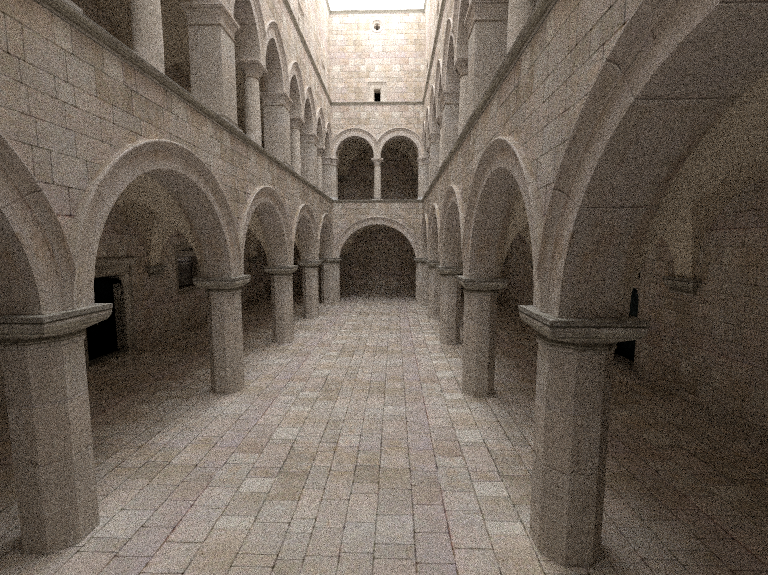
\includegraphics[width=0.20\linewidth]{imgs/hw_4_1d.png}
    \includegraphics[width=0.20\linewidth]{imgs/hw_4_1e.png}
    \caption{References for Homework 4.1.}
    \label{fig:hw_4_1}
\end{figure}

%\bibliographystyle{plain}
%\bibliography{refs}

\end{document}
